%% Short form of docs/compressed_partial_assembly/main.tex for PASC27 (ACM sigconf, 10 pages without
%% references).  Figures and tables are shared with the long form (../figures, ../tables); every
%% measured number arrives through ../tables/results_macros.tex or a generated table.  Build: make.
%% Review copy: `anonymous` hides the author block and the self-citation; drop it for the final
%% version, which also takes the ACM rights block in place of the \setcopyright{none} below.
\documentclass[sigconf,review,anonymous]{acmart}

\usepackage{booktabs}

\newcommand{\MachineBandwidth}{403}
\newcommand{\MachineNominalBandwidth}{500}
\newcommand{\MachineBandwidthPct}{81}
\newcommand{\MachinePeakFsixtyfour}{3{,}571}
\newcommand{\MachinePeakFthirtytwo}{7{,}142}
\newcommand{\MeasuredDof}{2.74\times10^{6}}
\newcommand{\BsrMeasuredSixtyfour}{575}
\newcommand{\BsrBoundSixtyfour}{574}
\newcommand{\BsrMeasuredThirtytwo}{1{,}029}
\newcommand{\BsrBoundThirtytwo}{1{,}064}
\newcommand{\nqTetFour}{1}
\newcommand{\rTetFour}{1}
\newcommand{\perpointTetFour}{45}
\newcommand{\minimalTetFour}{45}
\newcommand{\storeTetFour}{45}
\newcommand{\flopsTetFour}{192}
\newcommand{\directTetFour}{192}
\newcommand{\rankdiagTetFour}{1}
\newcommand{\rankoffTetFour}{1}
\newcommand{\blocksTetFour}{15}
\newcommand{\bsrsixtyfourTetFour}{383}
\newcommand{\bsrthirtytwoTetFour}{203}
\newcommand{\painteightTetFour}{98}
\newcommand{\pafsixteenTetFour}{188}
\newcommand{\ratiointTetFour}{3.9}
\newcommand{\ratiohalfTetFour}{2.0}
\newcommand{\exactQpPctTetFour}{44}
\newcommand{\exactEaPctTetFour}{62}
\newcommand{\exactBsrPctTetFour}{53}
\newcommand{\nqTetTen}{11}
\newcommand{\rTetTen}{4}
\newcommand{\perpointTetTen}{495}
\newcommand{\minimalTetTen}{450}
\newcommand{\storeTetTen}{450}
\newcommand{\flopsTetTen}{2856}
\newcommand{\directTetTen}{2991}
\newcommand{\rankdiagTetTen}{10}
\newcommand{\rankoffTetTen}{10}
\newcommand{\blocksTetTen}{29}
\newcommand{\bsrsixtyfourTetTen}{731}
\newcommand{\bsrthirtytwoTetTen}{386}
\newcommand{\painteightTetTen}{114}
\newcommand{\pafsixteenTetTen}{226}
\newcommand{\ratiointTetTen}{6.4}
\newcommand{\ratiohalfTetTen}{3.2}
\newcommand{\exactQpPctTetTen}{49}
\newcommand{\exactEaPctTetTen}{55}
\newcommand{\exactBsrPctTetTen}{52}
\newcommand{\nqHexEight}{8}
\newcommand{\rHexEight}{7}
\newcommand{\perpointHexEight}{360}
\newcommand{\minimalHexEight}{288}
\newcommand{\storeHexEight}{288}
\newcommand{\flopsHexEight}{1860}
\newcommand{\directHexEight}{2076}
\newcommand{\rankdiagHexEight}{4}
\newcommand{\rankoffHexEight}{8}
\newcommand{\blocksHexEight}{27}
\newcommand{\bsrsixtyfourHexEight}{687}
\newcommand{\bsrthirtytwoHexEight}{363}
\newcommand{\painteightHexEight}{97}
\newcommand{\pafsixteenHexEight}{193}
\newcommand{\ratiointHexEight}{7.1}
\newcommand{\ratiohalfHexEight}{3.6}
\newcommand{\exactQpPctHexEight}{56}
\newcommand{\exactEaPctHexEight}{56}
\newcommand{\exactBsrPctHexEight}{52}
\newcommand{\nqHexTwentySeven}{64}
\newcommand{\rHexTwentySeven}{26}
\newcommand{\perpointHexTwentySeven}{2880}
\newcommand{\minimalHexTwentySeven}{2592}
\newcommand{\storeHexTwentySeven}{2592}
\newcommand{\flopsHexTwentySeven}{21168}
\newcommand{\directHexTwentySeven}{70848}
\newcommand{\rankdiagHexTwentySeven}{48}
\newcommand{\rankoffHexTwentySeven}{64}
\newcommand{\blocksHexTwentySeven}{64}
\newcommand{\bsrsixtyfourHexTwentySeven}{1{,}624}
\newcommand{\bsrthirtytwoHexTwentySeven}{856}
\newcommand{\painteightHexTwentySeven}{108}
\newcommand{\pafsixteenHexTwentySeven}{216}
\newcommand{\ratiointHexTwentySeven}{15.0}
\newcommand{\ratiohalfHexTwentySeven}{7.5}
\newcommand{\exactQpPctHexTwentySeven}{50}
\newcommand{\exactEaPctHexTwentySeven}{52}
\newcommand{\exactBsrPctHexTwentySeven}{51}

\newcommand{\EaDiffEightMemVsSixtyFourHexEight}{8.1}
\newcommand{\EaDiffEightMemVsSixtyFourHexTwentySeven}{12.4}
\newcommand{\EaDiffEightMemVsSixtyFourTetFour}{3.3}
\newcommand{\EaDiffEightMemVsSixtyFourTetTen}{7.2}
\newcommand{\EaDiffEightMemVsThirtyTwoHexEight}{4.3}
\newcommand{\EaDiffEightMemVsThirtyTwoHexTwentySeven}{6.5}
\newcommand{\EaDiffEightMemVsThirtyTwoTetFour}{1.8}
\newcommand{\EaDiffEightMemVsThirtyTwoTetTen}{3.8}
\newcommand{\EaDiffEightRateHexEight}{1{,}976}
\newcommand{\EaDiffEightRateHexTwentySeven}{1{,}786}
\newcommand{\EaDiffEightRateTetFour}{1{,}303}
\newcommand{\EaDiffEightRateTetTen}{1{,}747}
\newcommand{\EaDiffEightVsSixtyFourHexEight}{3.32}
\newcommand{\EaDiffEightVsSixtyFourHexTwentySeven}{6.99}
\newcommand{\EaDiffEightVsSixtyFourTetFour}{1.31}
\newcommand{\EaDiffEightVsSixtyFourTetTen}{3.16}
\newcommand{\EaDiffEightVsThirtyTwoHexEight}{1.89}
\newcommand{\EaDiffEightVsThirtyTwoHexTwentySeven}{3.83}
\newcommand{\EaDiffEightVsThirtyTwoTetFour}{0.72}
\newcommand{\EaDiffEightVsThirtyTwoTetTen}{1.67}
\newcommand{\EaDiffHalfMemVsSixtyFourHexEight}{4.1}
\newcommand{\EaDiffHalfMemVsSixtyFourHexTwentySeven}{6.2}
\newcommand{\EaDiffHalfMemVsSixtyFourTetFour}{1.7}
\newcommand{\EaDiffHalfMemVsSixtyFourTetTen}{3.6}
\newcommand{\EaDiffHalfMemVsThirtyTwoHexEight}{2.1}
\newcommand{\EaDiffHalfMemVsThirtyTwoHexTwentySeven}{3.3}
\newcommand{\EaDiffHalfMemVsThirtyTwoTetFour}{0.9}
\newcommand{\EaDiffHalfMemVsThirtyTwoTetTen}{1.9}
\newcommand{\EaDiffHalfRateHexEight}{1{,}595}
\newcommand{\EaDiffHalfRateHexTwentySeven}{1{,}398}
\newcommand{\EaDiffHalfRateTetFour}{1{,}198}
\newcommand{\EaDiffHalfRateTetTen}{1{,}428}
\newcommand{\EaDiffHalfVsSixtyFourHexEight}{2.68}
\newcommand{\EaDiffHalfVsSixtyFourHexTwentySeven}{5.47}
\newcommand{\EaDiffHalfVsSixtyFourTetFour}{1.21}
\newcommand{\EaDiffHalfVsSixtyFourTetTen}{2.58}
\newcommand{\EaDiffHalfVsThirtyTwoHexEight}{1.53}
\newcommand{\EaDiffHalfVsThirtyTwoHexTwentySeven}{3.00}
\newcommand{\EaDiffHalfVsThirtyTwoTetFour}{0.66}
\newcommand{\EaDiffHalfVsThirtyTwoTetTen}{1.36}
\newcommand{\EaFullHalfMemVsSixtyFourHexEight}{3.4}
\newcommand{\EaFullHalfMemVsSixtyFourHexTwentySeven}{5.9}
\newcommand{\EaFullHalfMemVsSixtyFourTetFour}{1.2}
\newcommand{\EaFullHalfMemVsSixtyFourTetTen}{3.1}
\newcommand{\EaFullHalfMemVsThirtyTwoHexEight}{1.8}
\newcommand{\EaFullHalfMemVsThirtyTwoHexTwentySeven}{3.1}
\newcommand{\EaFullHalfMemVsThirtyTwoTetFour}{0.6}
\newcommand{\EaFullHalfMemVsThirtyTwoTetTen}{1.7}
\newcommand{\EaFullHalfRateHexEight}{1{,}359}
\newcommand{\EaFullHalfRateHexTwentySeven}{1{,}282}
\newcommand{\EaFullHalfRateTetFour}{824}
\newcommand{\EaFullHalfRateTetTen}{1{,}261}
\newcommand{\EaFullHalfVsSixtyFourHexEight}{2.28}
\newcommand{\EaFullHalfVsSixtyFourHexTwentySeven}{5.02}
\newcommand{\EaFullHalfVsSixtyFourTetFour}{0.83}
\newcommand{\EaFullHalfVsSixtyFourTetTen}{2.28}
\newcommand{\EaFullHalfVsThirtyTwoHexEight}{1.30}
\newcommand{\EaFullHalfVsThirtyTwoHexTwentySeven}{2.75}
\newcommand{\EaFullHalfVsThirtyTwoTetFour}{0.45}
\newcommand{\EaFullHalfVsThirtyTwoTetTen}{1.20}
\newcommand{\EaPairEightMemVsSixtyFourHexEight}{7.3}
\newcommand{\EaPairEightMemVsSixtyFourHexTwentySeven}{11.1}
\newcommand{\EaPairEightMemVsSixtyFourTetFour}{3.0}
\newcommand{\EaPairEightMemVsSixtyFourTetTen}{6.5}
\newcommand{\EaPairEightMemVsThirtyTwoHexEight}{3.8}
\newcommand{\EaPairEightMemVsThirtyTwoHexTwentySeven}{5.9}
\newcommand{\EaPairEightMemVsThirtyTwoTetFour}{1.6}
\newcommand{\EaPairEightMemVsThirtyTwoTetTen}{3.4}
\newcommand{\EaPairEightRateHexEight}{1{,}850}
\newcommand{\EaPairEightRateHexTwentySeven}{1{,}604}
\newcommand{\EaPairEightRateTetFour}{1{,}199}
\newcommand{\EaPairEightRateTetTen}{1{,}522}
\newcommand{\EaPairEightVsSixtyFourHexEight}{3.11}
\newcommand{\EaPairEightVsSixtyFourHexTwentySeven}{6.28}
\newcommand{\EaPairEightVsSixtyFourTetFour}{1.21}
\newcommand{\EaPairEightVsSixtyFourTetTen}{2.75}
\newcommand{\EaPairEightVsThirtyTwoHexEight}{1.77}
\newcommand{\EaPairEightVsThirtyTwoHexTwentySeven}{3.44}
\newcommand{\EaPairEightVsThirtyTwoTetFour}{0.66}
\newcommand{\EaPairEightVsThirtyTwoTetTen}{1.45}
\newcommand{\MfRateHexEight}{255}
\newcommand{\MfRateHexTwentySeven}{229}
\newcommand{\MfRateTetFour}{315}
\newcommand{\MfRateTetTen}{507}
\newcommand{\MfVsSixtyFourHexEight}{0.43}
\newcommand{\MfVsSixtyFourHexTwentySeven}{0.90}
\newcommand{\MfVsSixtyFourTetFour}{0.32}
\newcommand{\MfVsSixtyFourTetTen}{0.92}
\newcommand{\MfVsThirtyTwoHexEight}{0.24}
\newcommand{\MfVsThirtyTwoHexTwentySeven}{0.49}
\newcommand{\MfVsThirtyTwoTetFour}{0.17}
\newcommand{\MfVsThirtyTwoTetTen}{0.48}
\newcommand{\PzeroMemVsSixtyFourHexEight}{11.5}
\newcommand{\PzeroMemVsSixtyFourTetTen}{16.3}
\newcommand{\PzeroMemVsThirtyTwoHexEight}{6.1}
\newcommand{\PzeroMemVsThirtyTwoTetTen}{8.6}
\newcommand{\PzeroRateHexEight}{992}
\newcommand{\PzeroRateTetTen}{1{,}063}
\newcommand{\PzeroVsSixtyFourHexEight}{1.66}
\newcommand{\PzeroVsSixtyFourTetTen}{1.92}
\newcommand{\PzeroVsThirtyTwoHexEight}{0.95}
\newcommand{\PzeroVsThirtyTwoTetTen}{1.01}
\newcommand{\QbsrEightDiffMemVsSixtyFourHexEight}{4.6}
\newcommand{\QbsrEightDiffMemVsSixtyFourHexTwentySeven}{4.5}
\newcommand{\QbsrEightDiffMemVsSixtyFourTetFour}{4.7}
\newcommand{\QbsrEightDiffMemVsSixtyFourTetTen}{4.5}
\newcommand{\QbsrEightDiffMemVsThirtyTwoHexEight}{2.4}
\newcommand{\QbsrEightDiffMemVsThirtyTwoHexTwentySeven}{2.4}
\newcommand{\QbsrEightDiffMemVsThirtyTwoTetFour}{2.5}
\newcommand{\QbsrEightDiffMemVsThirtyTwoTetTen}{2.4}
\newcommand{\QbsrEightDiffRateHexEight}{1{,}881}
\newcommand{\QbsrEightDiffRateHexTwentySeven}{748}
\newcommand{\QbsrEightDiffRateTetFour}{3{,}371}
\newcommand{\QbsrEightDiffRateTetTen}{1{,}714}
\newcommand{\QbsrEightDiffVsSixtyFourHexEight}{3.16}
\newcommand{\QbsrEightDiffVsSixtyFourHexTwentySeven}{2.93}
\newcommand{\QbsrEightDiffVsSixtyFourTetFour}{3.40}
\newcommand{\QbsrEightDiffVsSixtyFourTetTen}{3.10}
\newcommand{\QbsrEightDiffVsThirtyTwoHexEight}{1.80}
\newcommand{\QbsrEightDiffVsThirtyTwoHexTwentySeven}{1.60}
\newcommand{\QbsrEightDiffVsThirtyTwoTetFour}{1.86}
\newcommand{\QbsrEightDiffVsThirtyTwoTetTen}{1.64}
\newcommand{\QbsrEightFullMemVsSixtyFourHexEight}{4.4}
\newcommand{\QbsrEightFullMemVsSixtyFourHexTwentySeven}{4.4}
\newcommand{\QbsrEightFullMemVsSixtyFourTetFour}{4.4}
\newcommand{\QbsrEightFullMemVsSixtyFourTetTen}{4.3}
\newcommand{\QbsrEightFullMemVsThirtyTwoHexEight}{2.3}
\newcommand{\QbsrEightFullMemVsThirtyTwoHexTwentySeven}{2.3}
\newcommand{\QbsrEightFullMemVsThirtyTwoTetFour}{2.3}
\newcommand{\QbsrEightFullMemVsThirtyTwoTetTen}{2.3}
\newcommand{\QbsrEightFullRateHexEight}{1{,}851}
\newcommand{\QbsrEightFullRateHexTwentySeven}{772}
\newcommand{\QbsrEightFullRateTetFour}{3{,}107}
\newcommand{\QbsrEightFullRateTetTen}{1{,}675}
\newcommand{\QbsrEightFullVsSixtyFourHexEight}{3.11}
\newcommand{\QbsrEightFullVsSixtyFourHexTwentySeven}{3.02}
\newcommand{\QbsrEightFullVsSixtyFourTetFour}{3.14}
\newcommand{\QbsrEightFullVsSixtyFourTetTen}{3.03}
\newcommand{\QbsrEightFullVsThirtyTwoHexEight}{1.77}
\newcommand{\QbsrEightFullVsThirtyTwoHexTwentySeven}{1.65}
\newcommand{\QbsrEightFullVsThirtyTwoTetFour}{1.71}
\newcommand{\QbsrEightFullVsThirtyTwoTetTen}{1.60}
\newcommand{\QbsrEightMemVsSixtyFourHexEight}{9.6}
\newcommand{\QbsrEightMemVsSixtyFourHexTwentySeven}{9.2}
\newcommand{\QbsrEightMemVsSixtyFourTetFour}{9.8}
\newcommand{\QbsrEightMemVsSixtyFourTetTen}{9.1}
\newcommand{\QbsrEightMemVsThirtyTwoHexEight}{5.1}
\newcommand{\QbsrEightMemVsThirtyTwoHexTwentySeven}{4.8}
\newcommand{\QbsrEightMemVsThirtyTwoTetFour}{5.2}
\newcommand{\QbsrEightMemVsThirtyTwoTetTen}{4.8}
\newcommand{\QbsrEightRateHexEight}{2{,}122}
\newcommand{\QbsrEightRateHexTwentySeven}{847}
\newcommand{\QbsrEightRateTetFour}{3{,}874}
\newcommand{\QbsrEightRateTetTen}{1{,}906}
\newcommand{\QbsrEightUpperIdxMemVsSixtyFourHexEight}{8.6}
\newcommand{\QbsrEightUpperIdxMemVsSixtyFourHexTwentySeven}{8.2}
\newcommand{\QbsrEightUpperIdxMemVsSixtyFourTetFour}{8.8}
\newcommand{\QbsrEightUpperIdxMemVsSixtyFourTetTen}{8.2}
\newcommand{\QbsrEightUpperIdxMemVsThirtyTwoHexEight}{4.6}
\newcommand{\QbsrEightUpperIdxMemVsThirtyTwoHexTwentySeven}{4.3}
\newcommand{\QbsrEightUpperIdxMemVsThirtyTwoTetFour}{4.6}
\newcommand{\QbsrEightUpperIdxMemVsThirtyTwoTetTen}{4.3}
\newcommand{\QbsrEightUpperIdxRateHexEight}{2{,}154}
\newcommand{\QbsrEightUpperIdxRateHexTwentySeven}{831}
\newcommand{\QbsrEightUpperIdxRateTetFour}{3{,}803}
\newcommand{\QbsrEightUpperIdxRateTetTen}{1{,}920}
\newcommand{\QbsrEightUpperIdxVsSixtyFourHexEight}{3.62}
\newcommand{\QbsrEightUpperIdxVsSixtyFourHexTwentySeven}{3.25}
\newcommand{\QbsrEightUpperIdxVsSixtyFourTetFour}{3.84}
\newcommand{\QbsrEightUpperIdxVsSixtyFourTetTen}{3.47}
\newcommand{\QbsrEightUpperIdxVsThirtyTwoHexEight}{2.06}
\newcommand{\QbsrEightUpperIdxVsThirtyTwoHexTwentySeven}{1.78}
\newcommand{\QbsrEightUpperIdxVsThirtyTwoTetFour}{2.10}
\newcommand{\QbsrEightUpperIdxVsThirtyTwoTetTen}{1.83}
\newcommand{\QbsrEightVsSixtyFourHexEight}{3.56}
\newcommand{\QbsrEightVsSixtyFourHexTwentySeven}{3.32}
\newcommand{\QbsrEightVsSixtyFourTetFour}{3.91}
\newcommand{\QbsrEightVsSixtyFourTetTen}{3.45}
\newcommand{\QbsrEightVsThirtyTwoHexEight}{2.03}
\newcommand{\QbsrEightVsThirtyTwoHexTwentySeven}{1.82}
\newcommand{\QbsrEightVsThirtyTwoTetFour}{2.14}
\newcommand{\QbsrEightVsThirtyTwoTetTen}{1.82}
\newcommand{\QbsrHalfMemVsSixtyFourHexEight}{7.4}
\newcommand{\QbsrHalfMemVsSixtyFourHexTwentySeven}{7.0}
\newcommand{\QbsrHalfMemVsSixtyFourTetFour}{7.5}
\newcommand{\QbsrHalfMemVsSixtyFourTetTen}{7.0}
\newcommand{\QbsrHalfMemVsThirtyTwoHexEight}{3.9}
\newcommand{\QbsrHalfMemVsThirtyTwoHexTwentySeven}{3.7}
\newcommand{\QbsrHalfMemVsThirtyTwoTetFour}{4.0}
\newcommand{\QbsrHalfMemVsThirtyTwoTetTen}{3.7}
\newcommand{\QbsrHalfRateHexEight}{1{,}961}
\newcommand{\QbsrHalfRateHexTwentySeven}{797}
\newcommand{\QbsrHalfRateTetFour}{3{,}643}
\newcommand{\QbsrHalfRateTetTen}{1{,}685}
\newcommand{\QbsrHalfVsSixtyFourHexEight}{3.29}
\newcommand{\QbsrHalfVsSixtyFourHexTwentySeven}{3.12}
\newcommand{\QbsrHalfVsSixtyFourTetFour}{3.68}
\newcommand{\QbsrHalfVsSixtyFourTetTen}{3.05}
\newcommand{\QbsrHalfVsThirtyTwoHexEight}{1.88}
\newcommand{\QbsrHalfVsThirtyTwoHexTwentySeven}{1.71}
\newcommand{\QbsrHalfVsThirtyTwoTetFour}{2.01}
\newcommand{\QbsrHalfVsThirtyTwoTetTen}{1.61}
\newcommand{\QpEightMdMemVsSixtyFourHexEight}{3.8}
\newcommand{\QpEightMdMemVsSixtyFourHexTwentySeven}{12.8}
\newcommand{\QpEightMdMemVsSixtyFourTetTen}{4.6}
\newcommand{\QpEightMdMemVsThirtyTwoHexEight}{2.0}
\newcommand{\QpEightMdMemVsThirtyTwoHexTwentySeven}{6.7}
\newcommand{\QpEightMdMemVsThirtyTwoTetTen}{2.4}
\newcommand{\QpEightMdRateHexEight}{951}
\newcommand{\QpEightMdRateHexTwentySeven}{1{,}036}
\newcommand{\QpEightMdRateTetTen}{952}
\newcommand{\QpEightMdVsSixtyFourHexEight}{1.60}
\newcommand{\QpEightMdVsSixtyFourHexTwentySeven}{4.05}
\newcommand{\QpEightMdVsSixtyFourTetTen}{1.72}
\newcommand{\QpEightMdVsThirtyTwoHexEight}{0.91}
\newcommand{\QpEightMdVsThirtyTwoHexTwentySeven}{2.22}
\newcommand{\QpEightMdVsThirtyTwoTetTen}{0.91}
\newcommand{\QpHalfMdMemVsSixtyFourHexEight}{2.3}
\newcommand{\QpHalfMdMemVsSixtyFourHexTwentySeven}{6.6}
\newcommand{\QpHalfMdMemVsSixtyFourTetTen}{2.7}
\newcommand{\QpHalfMdMemVsThirtyTwoHexEight}{1.2}
\newcommand{\QpHalfMdMemVsThirtyTwoHexTwentySeven}{3.5}
\newcommand{\QpHalfMdMemVsThirtyTwoTetTen}{1.4}
\newcommand{\QpHalfMdRateHexEight}{848}
\newcommand{\QpHalfMdRateHexTwentySeven}{985}
\newcommand{\QpHalfMdRateTetTen}{869}
\newcommand{\QpHalfMdVsSixtyFourHexEight}{1.42}
\newcommand{\QpHalfMdVsSixtyFourHexTwentySeven}{3.86}
\newcommand{\QpHalfMdVsSixtyFourTetTen}{1.57}
\newcommand{\QpHalfMdVsThirtyTwoHexEight}{0.81}
\newcommand{\QpHalfMdVsThirtyTwoHexTwentySeven}{2.11}
\newcommand{\QpHalfMdVsThirtyTwoTetTen}{0.83}
\newcommand{\QpHalfMemVsSixtyFourHexEight}{2.9}
\newcommand{\QpHalfMemVsSixtyFourHexTwentySeven}{6.8}
\newcommand{\QpHalfMemVsSixtyFourTetFour}{2.0}
\newcommand{\QpHalfMemVsSixtyFourTetTen}{3.3}
\newcommand{\QpHalfMemVsThirtyTwoHexEight}{1.5}
\newcommand{\QpHalfMemVsThirtyTwoHexTwentySeven}{3.6}
\newcommand{\QpHalfMemVsThirtyTwoTetFour}{1.1}
\newcommand{\QpHalfMemVsThirtyTwoTetTen}{1.7}
\newcommand{\QpHalfRateHexEight}{1{,}095}
\newcommand{\QpHalfRateHexTwentySeven}{1{,}101}
\newcommand{\QpHalfRateTetFour}{1{,}067}
\newcommand{\QpHalfRateTetTen}{1{,}094}
\newcommand{\QpHalfVsSixtyFourHexEight}{1.84}
\newcommand{\QpHalfVsSixtyFourHexTwentySeven}{4.31}
\newcommand{\QpHalfVsSixtyFourTetFour}{1.08}
\newcommand{\QpHalfVsSixtyFourTetTen}{1.98}
\newcommand{\QpHalfVsThirtyTwoHexEight}{1.05}
\newcommand{\QpHalfVsThirtyTwoHexTwentySeven}{2.36}
\newcommand{\QpHalfVsThirtyTwoTetFour}{0.59}
\newcommand{\QpHalfVsThirtyTwoTetTen}{1.04}
\newcommand{\SetupBsrSixtyFourHexEight}{382}
\newcommand{\SetupBsrSixtyFourHexTwentySeven}{966}
\newcommand{\SetupBsrSixtyFourTetFour}{344}
\newcommand{\SetupBsrSixtyFourTetTen}{462}
\newcommand{\SetupBsrThirtyTwoHexEight}{323}
\newcommand{\SetupBsrThirtyTwoHexTwentySeven}{834}
\newcommand{\SetupBsrThirtyTwoTetFour}{311}
\newcommand{\SetupBsrThirtyTwoTetTen}{399}
\newcommand{\SetupEaDiffHalfHexEight}{138}
\newcommand{\SetupEaDiffHalfHexTwentySeven}{421}
\newcommand{\SetupEaDiffHalfTetFour}{91}
\newcommand{\SetupEaDiffHalfTetTen}{271}
\newcommand{\SetupPzeroHexEight}{61}
\newcommand{\SetupPzeroTetTen}{67}
\newcommand{\SetupQbsrEightDiffHexEight}{384}
\newcommand{\SetupQbsrEightDiffHexTwentySeven}{1{,}187}
\newcommand{\SetupQbsrEightDiffTetFour}{349}
\newcommand{\SetupQbsrEightDiffTetTen}{518}
\newcommand{\SetupQbsrEightHexEight}{358}
\newcommand{\SetupQbsrEightHexTwentySeven}{898}
\newcommand{\SetupQbsrEightTetFour}{329}
\newcommand{\SetupQbsrEightTetTen}{437}
\newcommand{\SetupQpHalfHexEight}{104}
\newcommand{\SetupQpHalfHexTwentySeven}{129}
\newcommand{\SetupQpHalfTetFour}{78}
\newcommand{\SetupQpHalfTetTen}{187}
\newcommand{\bsrSixtyFourRateHexEight}{596}
\newcommand{\bsrSixtyFourRateHexTwentySeven}{255}
\newcommand{\bsrSixtyFourRateTetFour}{991}
\newcommand{\bsrSixtyFourRateTetTen}{553}
\newcommand{\bsrThirtyTwoRateHexEight}{1{,}044}
\newcommand{\bsrThirtyTwoRateHexTwentySeven}{466}
\newcommand{\bsrThirtyTwoRateTetFour}{1{,}814}
\newcommand{\bsrThirtyTwoRateTetTen}{1{,}047}
\newcommand{\corrQpSixtyFourHexEight}{$2.2\times10^{-16}$}
\newcommand{\corrQpSixtyFourHexTwentySeven}{$2.4\times10^{-6}$}
\newcommand{\corrQpSixtyFourTetFour}{$1.9\times10^{-16}$}
\newcommand{\corrQpSixtyFourTetTen}{$1.5\times10^{-6}$}
\newcommand{\errEaDiffEightHexEight}{$5.5\times10^{-5}$}
\newcommand{\errEaDiffEightHexTwentySeven}{$1.2\times10^{-2}$}
\newcommand{\errEaDiffEightTetFour}{$1.8\times10^{-4}$}
\newcommand{\errEaDiffEightTetTen}{$5.5\times10^{-4}$}
\newcommand{\errEaDiffHalfHexEight}{$7.4\times10^{-8}$}
\newcommand{\errEaDiffHalfHexTwentySeven}{$2.6\times10^{-8}$}
\newcommand{\errEaDiffHalfTetFour}{$4.3\times10^{-6}$}
\newcommand{\errEaDiffHalfTetTen}{$2.5\times10^{-6}$}
\newcommand{\errEaPairEightHexEight}{$6.0\times10^{-5}$}
\newcommand{\errEaPairEightHexTwentySeven}{$6.7\times10^{-6}$}
\newcommand{\errEaPairEightTetFour}{$3.2\times10^{-5}$}
\newcommand{\errEaPairEightTetTen}{$2.3\times10^{-5}$}
\newcommand{\fullEightFailed}{9}
\newcommand{\fullEightTried}{9}
\newcommand{\gbsBsrThirtyTwoHexEight}{372}
\newcommand{\gbsBsrThirtyTwoHexTwentySeven}{393}
\newcommand{\gbsBsrThirtyTwoTetFour}{361}
\newcommand{\gbsBsrThirtyTwoTetTen}{398}
\newcommand{\gbsQbsrEightHexEight}{149}
\newcommand{\gbsQbsrEightHexTwentySeven}{148}
\newcommand{\gbsQbsrEightTetFour}{149}
\newcommand{\gbsQbsrEightTetTen}{151}
\newcommand{\newtonDofHexEight}{1{,}073{,}733}
\newcommand{\newtonDofHexTwentySeven}{1{,}073{,}733}
\newcommand{\newtonDofTetFour}{1{,}082{,}427}
\newcommand{\newtonDofTetTen}{1{,}082{,}427}
\newcommand{\newtonEaDiffEightHexEight}{17}
\newcommand{\newtonEaDiffEightHexTwentySeven}{694}
\newcommand{\newtonEaDiffEightTetFour}{16}
\newcommand{\newtonEaDiffEightTetTen}{110}
\newcommand{\newtonEaDiffHalfHexEight}{13}
\newcommand{\newtonEaDiffHalfHexTwentySeven}{24}
\newcommand{\newtonEaDiffHalfTetFour}{12}
\newcommand{\newtonEaDiffHalfTetTen}{48}
\newcommand{\newtonEaPairEightHexEight}{16}
\newcommand{\newtonEaPairEightHexTwentySeven}{32}
\newcommand{\newtonEaPairEightTetFour}{17}
\newcommand{\newtonEaPairEightTetTen}{64}
\newcommand{\newtonExactHexEight}{13}
\newcommand{\newtonExactHexTwentySeven}{24}
\newcommand{\newtonExactTetFour}{12}
\newcommand{\newtonExactTetTen}{48}
\newcommand{\newtonPzeroExtraHexEight}{23}
\newcommand{\newtonPzeroExtraTetFour}{0}
\newcommand{\newtonPzeroExtraTetTen}{54}
\newcommand{\newtonPzeroHexEight}{16}
\newcommand{\newtonPzeroTetFour}{12}
\newcommand{\newtonPzeroTetTen}{74}
\newcommand{\newtonQbsrEightHexEight}{16}
\newcommand{\newtonQbsrEightHexTwentySeven}{32}
\newcommand{\newtonQbsrEightTetFour}{16}
\newcommand{\newtonQbsrEightTetTen}{64}
\newcommand{\newtonQbsrHalfHexEight}{13}
\newcommand{\newtonQbsrHalfHexTwentySeven}{24}
\newcommand{\newtonQbsrHalfTetFour}{13}
\newcommand{\newtonQbsrHalfTetTen}{48}
\newcommand{\newtonQpEightElHexEight}{20}
\newcommand{\newtonQpEightElHexTwentySeven}{43}
\newcommand{\newtonQpEightElTetFour}{20}
\newcommand{\newtonQpEightElTetTen}{124}
\newcommand{\newtonQpEightMdHexEight}{13}
\newcommand{\newtonQpEightMdHexTwentySeven}{24}
\newcommand{\newtonQpEightMdTetTen}{48}
\newcommand{\offsetSavingHexEight}{10}
\newcommand{\offsetSavingHexTwentySeven}{10}
\newcommand{\offsetSavingTetFour}{10}
\newcommand{\offsetSavingTetTen}{10}
\newcommand{\pairErrGainHexEight}{1}
\newcommand{\pairErrGainHexTwentySeven}{1766}
\newcommand{\pairErrGainTetFour}{6}
\newcommand{\pairErrGainTetTen}{24}
\newcommand{\pairSlowdownHexEight}{6}
\newcommand{\pairSlowdownHexTwentySeven}{10}
\newcommand{\pairSlowdownTetFour}{8}
\newcommand{\pairSlowdownTetTen}{13}
\newcommand{\peakBsrThirtyTwoHexEight}{6.6}
\newcommand{\peakBsrThirtyTwoTetFour}{5.6}
\newcommand{\peakDofHexEight}{10{,}328{,}853}
\newcommand{\peakDofTetFour}{10{,}498{,}683}
\newcommand{\peakEaDiffHalfHexEight}{2.6}
\newcommand{\peakEaPairEightHexEight}{1.9}
\newcommand{\peakEaPairEightTetFour}{4.6}
\newcommand{\peakPzeroHexEight}{0.9}
\newcommand{\peakPzeroTetFour}{6.4}
\newcommand{\peakQbsrEightHexEight}{7.2}
\newcommand{\peakQbsrEightTetFour}{6.2}
\newcommand{\peakQbsrHalfHexEight}{7.3}
\newcommand{\peakQbsrHalfTetFour}{6.2}
\newcommand{\remainderShareHi}{8}
\newcommand{\remainderShareLo}{5}
\newcommand{\storeEaDiffHalfHexEight}{1.60}
\newcommand{\storeEaPairEightHexEight}{0.89}
\newcommand{\storeEaPairEightTetFour}{1.24}
\newcommand{\storeQbsrEightHexEight}{0.67}
\newcommand{\storeQbsrEightTetFour}{0.39}
\newcommand{\storeQbsrHalfHexEight}{0.88}
\newcommand{\storeQbsrHalfTetFour}{0.50}
\newcommand{\tenmNewtonExactHexEight}{16}
\newcommand{\tenmNewtonExactHexTwentySeven}{48}
\newcommand{\tenmNewtonExactTetFour}{19}
\newcommand{\tenmNewtonExactTetTen}{99}
\newcommand{\tenmNewtonQbsrEightHexEight}{16}
\newcommand{\tenmNewtonQbsrEightHexTwentySeven}{64}
\newcommand{\tenmNewtonQbsrEightTetFour}{20}
\newcommand{\tenmNewtonQbsrEightTetTen}{171}
\newcommand{\tenmNewtonQbsrHalfHexEight}{16}
\newcommand{\tenmNewtonQbsrHalfHexTwentySeven}{48}
\newcommand{\tenmNewtonQbsrHalfTetFour}{18}
\newcommand{\tenmNewtonQbsrHalfTetTen}{117}
\newcommand{\timeBsrSixtyFourHexEight}{1.68}
\newcommand{\timeBsrSixtyFourHexTwentySeven}{1.77}
\newcommand{\timeBsrSixtyFourTetFour}{1.36}
\newcommand{\timeBsrSixtyFourTetTen}{1.75}
\newcommand{\timeDofHexEight}{10{,}328{,}853}
\newcommand{\timeDofHexTwentySeven}{10{,}328{,}853}
\newcommand{\timeDofTetFour}{10{,}498{,}683}
\newcommand{\timeDofTetTen}{10{,}498{,}683}
\newcommand{\timeEaDiffHalfHexEight}{0.77}
\newcommand{\timeEaDiffHalfHexTwentySeven}{0.54}
\newcommand{\timeEaDiffHalfTetFour}{1.22}
\newcommand{\timeEaDiffHalfTetTen}{0.89}
\newcommand{\timeEaPairEightHexEight}{0.68}
\newcommand{\timeEaPairEightHexTwentySeven}{0.43}
\newcommand{\timeEaPairEightTetFour}{0.94}
\newcommand{\timeEaPairEightTetTen}{1.04}
\newcommand{\timeQbsrEightHexEight}{0.61}
\newcommand{\timeQbsrEightHexTwentySeven}{0.68}
\newcommand{\timeQbsrEightTetFour}{0.53}
\newcommand{\timeQbsrEightTetTen}{0.99}
\newcommand{\timeQbsrHalfHexEight}{0.67}
\newcommand{\timeQbsrHalfHexTwentySeven}{0.81}
\newcommand{\timeQbsrHalfTetFour}{0.46}
\newcommand{\timeQbsrHalfTetTen}{0.80}
\newcommand{\timeQpEightMdHexEight}{1.03}
\newcommand{\timeQpEightMdHexTwentySeven}{0.51}
\newcommand{\timeQpEightMdTetTen}{1.18}
\newcommand{\timeQpHalfHexEight}{1.00}
\newcommand{\timeQpHalfHexTwentySeven}{0.52}
\newcommand{\timeQpHalfTetFour}{0.98}
\newcommand{\timeQpHalfTetTen}{1.22}
\newcommand{\twistEaDiffEightHexEight}{81}
\newcommand{\twistEaDiffEightHexTwentySeven}{566}
\newcommand{\twistEaDiffEightTetFour}{391}
\newcommand{\twistEaDiffEightTetTen}{713}
\newcommand{\twistEaDiffHalfHexEight}{64}
\newcommand{\twistEaDiffHalfHexTwentySeven}{97}
\newcommand{\twistEaDiffHalfTetFour}{195}
\newcommand{\twistEaDiffHalfTetTen}{273}
\newcommand{\twistEaPairEightHexEight}{64}
\newcommand{\twistEaPairEightHexTwentySeven}{103}
\newcommand{\twistEaPairEightTetFour}{471}
\newcommand{\twistEaPairEightTetTen}{454}
\newcommand{\twistExactHexEight}{64}
\newcommand{\twistExactHexTwentySeven}{94}
\newcommand{\twistExactTetFour}{195}
\newcommand{\twistExactTetTen}{273}
\newcommand{\twistQbsrEightHexEight}{75}
\newcommand{\twistQbsrEightHexTwentySeven}{106}
\newcommand{\twistQbsrEightTetFour}{419}
\newcommand{\twistQbsrEightTetTen}{587}
\newcommand{\twistQbsrHalfHexEight}{64}
\newcommand{\twistQbsrHalfHexTwentySeven}{98}
\newcommand{\twistQbsrHalfTetFour}{195}
\newcommand{\twistQbsrHalfTetTen}{273}
\newcommand{\twistQpEightElHexEight}{82}
\newcommand{\twistQpEightElHexTwentySeven}{114}
\newcommand{\twistQpEightElTetFour}{367}
\newcommand{\twistQpEightElTetTen}{816}
\newcommand{\twistQpEightMdHexEight}{64}
\newcommand{\twistQpEightMdHexTwentySeven}{91}
\newcommand{\twistQpEightMdTetTen}{273}
\newcommand{\twistTimeEaDiffHalfHexEight}{0.80}
\newcommand{\twistTimeEaDiffHalfHexTwentySeven}{0.49}
\newcommand{\twistTimeEaDiffHalfTetFour}{1.99}
\newcommand{\twistTimeEaDiffHalfTetTen}{0.86}
\newcommand{\twistTimeEaPairEightHexEight}{0.68}
\newcommand{\twistTimeEaPairEightHexTwentySeven}{0.33}
\newcommand{\twistTimeEaPairEightTetFour}{3.25}
\newcommand{\twistTimeEaPairEightTetTen}{0.79}
\newcommand{\twistTimeQbsrEightHexEight}{0.93}
\newcommand{\twistTimeQbsrEightHexTwentySeven}{0.55}
\newcommand{\twistTimeQbsrEightTetFour}{1.23}
\newcommand{\twistTimeQbsrEightTetTen}{0.92}
\newcommand{\twistTimeQbsrHalfHexEight}{0.79}
\newcommand{\twistTimeQbsrHalfHexTwentySeven}{0.67}
\newcommand{\twistTimeQbsrHalfTetFour}{0.92}
\newcommand{\twistTimeQbsrHalfTetTen}{0.79}
\newcommand{\upperGainHexEight}{1.15}
\newcommand{\upperGainHexTwentySeven}{1.11}
\newcommand{\upperGainTetFour}{1.13}
\newcommand{\upperGainTetTen}{1.12}
\newcommand{\upperMemHexEight}{1.9}
\newcommand{\upperMemHexTwentySeven}{1.8}
\newcommand{\upperMemTetFour}{1.9}
\newcommand{\upperMemTetTen}{1.8}

\newcommand{\benchdofTetFour}{10{,}328{,}853}
\newcommand{\benchnTetFour}{150}
\newcommand{\benchdofTetTen}{10{,}328{,}853}
\newcommand{\benchnTetTen}{75}
\newcommand{\benchdofHexEight}{10{,}328{,}853}
\newcommand{\benchnHexEight}{150}
\newcommand{\benchdofHexTwentySeven}{10{,}328{,}853}
\newcommand{\benchnHexTwentySeven}{75}

\graphicspath{{../figures/}}
\makeatletter
\newcommand{\rows}[1]{\@@input #1 }
\makeatother

\newcommand{\xhat}{\boldsymbol{\xi}}
\newcommand{\Sq}{\widehat{S}^{q}}
\newcommand{\Sbar}{\overline{S}}
\newcommand{\Mab}{M^{ab}}
\newcommand{\eps}{\varepsilon}

%% Submission: no ACM rights block yet.
\setcopyright{none}
\settopmatter{printacmref=false}
\renewcommand\footnotetextcopyrightpermission[1]{}
\acmConference[PASC '27]{Platform for Advanced Scientific Computing Conference}{2027}{}

\begin{document}

\title{Compressed Operator Formats for Newton--Krylov Hyperelasticity: Quadrature Points, Element
Matrices and Sparse Matrices Compared}

\author{Patrick Zulian}
\orcid{0000-0002-5822-3288}
\affiliation{%
  \institution{Euler Institute, Universit\`a della Svizzera italiana}
  \city{Lugano}
  \country{Switzerland}}
\affiliation{%
  \institution{UniDistance Suisse}
  \city{Brig}
  \country{Switzerland}}
\affiliation{%
  \institution{University of Victoria}
  \city{Victoria}
  \state{British Columbia}
  \country{Canada}}
\email{patrick.zulian@usi.ch}

\begin{abstract}
Newton--Krylov solvers for finite-strain elasticity spend most of their time applying the tangent
operator, and how that operator is stored decides both the time and the memory of a solve.  We
evaluate compressed formats along the whole range from the assembled matrix to matrix-free
application: block sparse (BSR) matrices quantized per block, element matrices quantized per node
pair, and partial assembly that stores the pulled-back material tangent at the quadrature points
(on quadratic tetrahedra its $P_2$ moments, all the quadrature sees), against BSR in double and
single precision.  The formats share \texttt{fp16} and \texttt{int8} encodings decoded inside the
application, and a difference form that keeps rigid translations in the kernel of the encoded
element and assembled matrices whatever the rounding.  An encoding error enters inexact Newton as an
additive forcing term; half precision and \texttt{int8} mean-plus-deviation keep the exact
iteration counts, \texttt{int8} with one scale per element does not, and the quantized matrix fails
without the difference form.  On a 72-core Arm Neoverse-V2 CPU at $10^7$ degrees of freedom, for
linear and quadratic tetrahedra and trilinear and triquadratic hexahedra, the quantized sparse matrix
is the fastest format on tetrahedra, solving in $\timeQbsrHalfTetFour$--$\timeQbsrHalfTetTen$ of the
time of single-precision BSR from $\QbsrHalfMemVsThirtyTwoTetTen$--$\QbsrHalfMemVsThirtyTwoTetFour\times$
less operator memory; element matrices come close to it on trilinear and are ahead on triquadratic
hexahedra, and they keep the lowest peak memory, since they need no assembled matrix.
\end{abstract}

%% CCS concepts: take the XML from the ACM CCS tool for the final version.
\ccsdesc[500]{Mathematics of computing~Mathematical software performance}
\ccsdesc[300]{Mathematics of computing~Partial differential equations}
\ccsdesc[300]{Computing methodologies~Massively parallel and high-performance simulations}

\keywords{operator formats, quantization, mixed precision, partial assembly, element matrices,
sparse matrix--vector product, finite-strain elasticity, inexact Newton, Arm Neoverse V2}

\maketitle

%% ===================================================================================================
\section{Introduction}

Newton--Krylov solvers for finite-strain elasticity apply the tangent operator tens to hundreds of
times per Newton step.  Three families of formats compete for that operator.  An assembled matrix,
in block sparse row (BSR) form for a vector problem, pays one assembly per step and then applies at
the speed of memory: on the machine used here a BSR product sustains $\MachineBandwidth$~GB/s,
$81\%$ of the nominal bandwidth.  Element matrices store each element's dense block and apply it
with a gather and a scatter.  Partial assembly stores less --- the material tangent at the
quadrature points, or an average of it --- and applies it by a contraction with the reference
element; at the far end, a matrix-free application re-evaluates the constitutive law every time.
Moving along this range trades stored bytes against arithmetic, and quantizing the stored numbers
shifts the trade for every format at once.

The question this paper answers is which format, with which encoding, gives the shortest time to
solution and the smallest memory for a Newton--Krylov hyperelasticity solve, and why.  The answer
depends on three things the formats share: the bytes each streams per degree of freedom, the
arithmetic and gathering each performs, and the perturbation each encoding makes to the tangent,
which the Newton iteration either absorbs or pays for in iterations.  An element-constant
projection of the tangent~\cite{ZulianPA}, the smallest partial-assembly store, already shows the
last effect: it costs $\newtonPzeroExtraHexEight\%$ more Newton iterations on trilinear hexahedra and
$\newtonPzeroExtraTetTen\%$ more on quadratic tetrahedra in our study.

The contributions are:
\begin{itemize}
\item a common framework for the formats: each is a store written once per Newton step and an
  application that decodes it in registers, under the same \texttt{fp16} and \texttt{int8}
  encodings, with an error model in which what matters is the absolute rounding on smooth, nearly
  rigid modes, and its consequence for inexact Newton --- the encoding error adds to the forcing
  term;
\item the difference form, which stores only off-diagonal node blocks and keeps rigid translations
  exactly in the kernel of an encoded element or assembled matrix, with a scale per node pair for
  element matrices and, for the assembled matrix, each pair of blocks stored once in a
  SELL-C-$\sigma$ layout applied without atomics;
\item a minimal exact quadrature-point store: the tangent at the points or, where fewer, its moments
  against products of gradient functions ($\storeTetTen$ numbers per quadratic tetrahedron against
  $\perpointTetTen$ point values);
\item an evaluation on one Grace CPU for four element types up to $10^7$ degrees of freedom:
  throughput, operator and peak memory, Newton iteration counts and time to solution against BSR
  in double and single precision, and the resulting choice of format per element.
\end{itemize}

%% ===================================================================================================
\section{Related work}

Storing geometric factors at quadrature points and applying an operator by contraction underlies
the matrix-free frameworks of deal.II~\cite{KronbichlerKormann2012}, MFEM~\cite{MFEM2021} and
libCEED~\cite{libCEED2021}.  For finite-strain hyperelasticity, Davydov et
al.~\cite{Davydov2020} compare caching levels up to the stress with the full spatial tangent and
find them faster than a sparse matrix above polynomial degree one; Brown et al.~\cite{Brown2022}
store $17$ to $31$ scalars per point; Schussnig et al.~\cite{Schussnig2025} and Wichrowski et
al.~\cite{Wichrowski2025} extend the storage levels to anisotropic and automatically differentiated
materials.  All store double-precision point values.  Storage precision decoupled from arithmetic
precision is established in sparse linear algebra~\cite{Anzt2019,Gruetzmacher2023,HighamMary2022};
for sparse matrix--vector products the precision has been chosen per non-zero~\cite{Ahmad2019} or
per row~\cite{Tezcan2022} among floating-point formats, and matrix-free multigrid runs in single
precision inside a double-precision iteration~\cite{KronbichlerLjungkvist2019}.  Fixed-rate
compression~\cite{Lindstrom2014} and microscaling formats~\cite{Rouhani2023} share a scale per small
block.  We found no comparison of quantized formats across the assembled, element and quadrature
levels, no quantization of a stiffness matrix to eight bits, and no encoding that keeps the rigid
translations in the kernel of the encoded operator.  Inexact Newton methods converge at a rate set
by the forcing term~\cite{DemboEisenstatSteihaug1982}, to which a Jacobian error
adds~\cite{Kelley2018}.

%% ===================================================================================================
\section{Formats}

All formats represent the same element action.  For reference basis $\{\varphi_p\}$, quadrature
points $\xhat_q$ with weights $w_q$, and a hyperelastic tangent $A_{ijkl}=\partial P_{ij}/\partial
F_{kl}$~\cite{BonetWood2008}, the pulled-back tangent with the weight folded in is $\Sq_{ikmn} =
w_q\sum_{j,l} A_{ijkl}\,J^{-1}_{nj} J^{-1}_{ml}\det J$ at $\xhat_q$, and
\begin{equation}
  (\mathcal{H} h)_{ip} = \sum_{q}\sum_{k,m,n} \Sq_{ikmn}\, \partial_m h_k(\xhat_q)\,
  \partial_n\varphi_p(\xhat_q) .
  \label{eq:action}
\end{equation}
The formats differ in how much of \eqref{eq:action} is precomputed once per Newton step and stored:
the tangent at the points (partial assembly), the element matrix it produces, or the assembled
matrix.

\subsection{Quadrature-point stores}

Everything in \eqref{eq:action} except $\Sq$ belongs to the reference element; with the major
symmetry of an energy each point carries $45$ numbers.  The tangent enters only through products
of reference gradients, so it is seen through its moments against the product spaces $\Pi_{mn}$ of
the gradient spaces, and whichever is smaller --- the $n_q$ point values or a basis of moments ---
reproduces \eqref{eq:action} exactly (Table~\ref{tab:stores}).  On quadratic tetrahedra (TET10) the
ten $P_2$ moments $\Mab=\sum_q\lambda_a(\xhat_q)\lambda_b(\xhat_q)\Sq$ replace the eleven points of
the degree-$4$ rule~\cite{Keast1986}; on trilinear (HEX8) and triquadratic (HEX27) hexahedra the
point values are minimal.  Replacing $\Sq$ by its element mean $\Sbar$ gives the projected store
of~\cite{ZulianPA}, $45$ numbers per element and a Kronecker-rank-one approximation of the element
operator; the exact store differs from it by the deviations $\Sq-w_q\Sbar$, which is what makes a
mean-and-deviation encoding natural.  The store is laid out per block of $V$ elements, ordered
point, component, lane (Figure~\ref{fig:fmtpoints}).

\begin{table}[t]
\centering
\small
\setlength{\tabcolsep}{3.5pt}
\begin{tabular}{lrrrrr}
\toprule
element & $n_q$ & rank & $\dim\Pi_{mn}$ & points & minimal \\
\midrule
\rows{../tables/stores.tex}
\bottomrule
\end{tabular}
\caption{Numbers per element of an exact quadrature-point store (symmetric tangent); ``rank'' is
that of the reference gradients.}
\label{tab:stores}
\end{table}

\begin{figure*}[t]
\centering
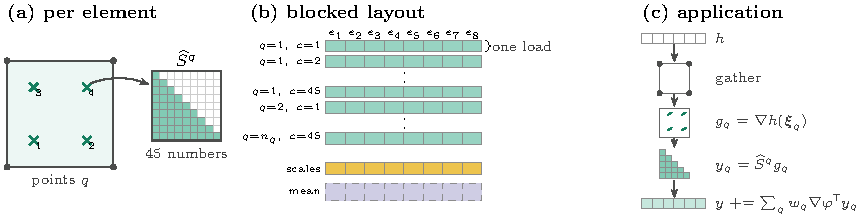
\includegraphics[width=0.92\textwidth]{fmt_points.pdf}
\caption{The quadrature-point store.  (a) The pulled-back tangent at a point, a symmetric $9\times9$
matrix of $45$ numbers.  (b) The blocked layout of $V$ elements: point, component, lane, one
vector load per component; a scale per element; the single-precision mean of the
mean-and-deviation encodings.  (c) The application, one element per vector lane.}
\Description{Three panels: an element with quadrature points and the stored tangent, the blocked
memory layout of codes, scales and means, and the steps of the application.}
\label{fig:fmtpoints}
\end{figure*}

\subsection{Element matrices in difference form}

Contracting the stored tensors with the basis derivatives once per Newton step gives each element's
$3N\times3N$ matrix, directly and without probing.  An element matrix annihilates rigid
translations, so each diagonal node block is minus the sum of its row's off-diagonal blocks.
Storing only $K_{pq}$, $p<q$, and applying $y_p=\sum_{q\ne p}K_{pq}(h_q-h_p)$ keeps the translations
in the kernel of the \emph{encoded} matrix whatever the rounding.  One \texttt{int8} scale per
element spends its range on the largest node-pair block, which on higher-order elements exceeds the
smallest by orders of magnitude; each pair therefore carries an $8$-bit factor
$r_{pq}=2^{-E}(1+m/8)\le1$ relative to the element scale $s_e$, $K_{pq}\approx s_e r_{pq}C_{pq}$
with $C_{pq}$ nine \texttt{int8} codes (Figure~\ref{fig:fmtelement}), as in microscaling
formats~\cite{Rouhani2023} with the node pair as the block.

\begin{figure*}[t]
\centering
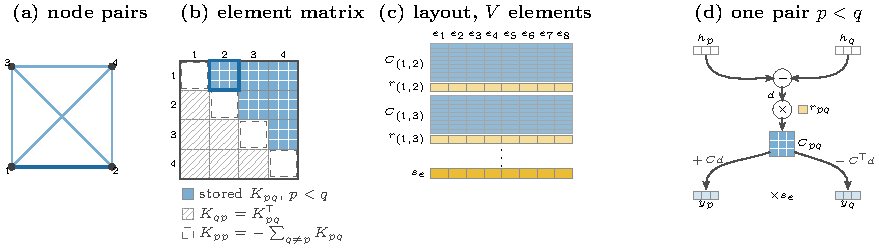
\includegraphics[width=0.92\textwidth]{fmt_element.pdf}
\caption{The element matrix in difference form with a scale per node pair.  (a) The $N(N-1)/2$
node pairs ($28$ on HEX8); the pair $(1,2)$ is framed in (b) and laid out in (c).  (b) Stored
off-diagonal blocks, their transposes and the diagonal blocks implied by the row sums.  (c) Layout
of a block of $V$ elements: nine \texttt{int8} codes $C_{pq}$ and a factor $r_{pq}$ per pair, a scale
$s_e$ per element.  (d) One pair, one element per vector lane; a translation, $h_q=h_p$, gives $d=0$
whatever the codes.}
\Description{Four panels: node pairs of an element, the stored upper blocks of the element matrix,
the memory layout of codes and scales for a block of elements, and the update of one node pair.}
\label{fig:fmtelement}
\end{figure*}

\subsection{Assembled matrices}

BSR stores each node coupling once, as a $3\times3$ block with a column index
(Figure~\ref{fig:fmtbsr}), where the element formats store it once per element sharing it.  We
quantize its blocks after the generated single-precision assembly, in \texttt{int8} with a
single-precision scale per block or in \texttt{fp16} with one power-of-two scale.  The rows of the
assembled tangent also annihilate translations, so the difference form holds with $p,q$ ranging over
the nodes and the diagonal blocks are neither stored nor indexed.  Each pair $i<j$ is stored once:
with $d=x_j-x_i$ the block adds $K_{ij}d$ to $y_i$ and $-K_{ij}^{\mathsf T}d$ to $y_j$, so the
encoded matrix is symmetric by construction, which the assembled one is only to the rounding of its
summation order.

Rows are held in the SELL-C-$\sigma$ format~\cite{Kreutzer2014}: $C=16$ rows side by side, sorted by
length within windows of $\sigma=32C$ rows and padded per group, so that one block position of $16$
rows is decoded as one vector; columns are $16$-bit offsets $j-i$ (Figure~\ref{fig:fmtqbsr}).  Each
thread owns whole windows and updates its own rows directly, lane after lane; blocks reaching beyond
its rows or the offsets go to a per-thread remainder whose updates of other threads' rows pass
through slots added after a barrier, so the product is deterministic and needs no atomics, where
symmetric products have otherwise been parallelised by colouring~\cite{Alappat2020,Elafrou2019}.  At
$10^7$ degrees of freedom on $72$ threads the remainder holds $\remainderShareLo$--$\remainderShareHi\%$
of the stored blocks.  The encoder writes the records ($13$ bytes per stored block in \texttt{int8}
against $36$ per assembled one) over the assembled values in rounds that never overwrite a value
not yet read.

\begin{figure*}[t]
\centering
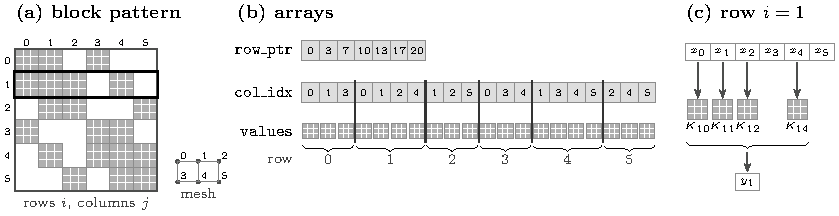
\includegraphics[width=0.92\textwidth]{fmt_bsr.pdf}
\caption{BSR.  (a) The block pattern of a six-node mesh; the framed row is the one of (c).  (b) Row
pointers, a column index per block and its nine values ($72$ bytes in \texttt{fp64}, $36$ in
\texttt{fp32}).  (c) One row of the product: each block streams once, $x_j$ is gathered per block.}
\Description{Three panels: the block pattern of a small sparse matrix, its row pointer, column index
and value arrays, and one row of the matrix-vector product.}
\label{fig:fmtbsr}
\end{figure*}

\begin{figure*}[t]
\centering
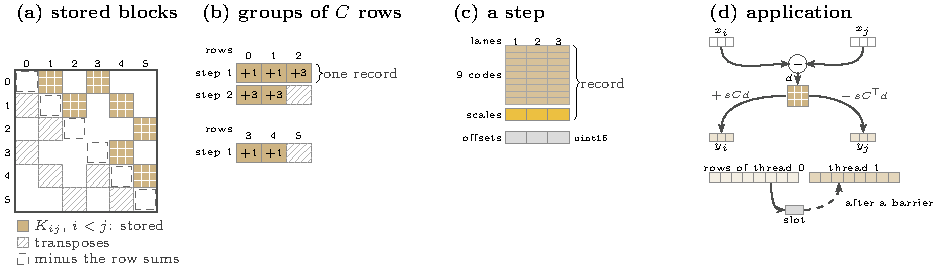
\includegraphics[width=0.92\textwidth]{fmt_qbsr.pdf}
\caption{The quantized assembled matrix, drawn with $C=3$ ($16$ in the code) on the mesh of
Figure~\ref{fig:fmtbsr}.  (a) Stored upper blocks; the diagonal blocks are minus the row sums.
(b) Rows in groups of $C$, sorted by length within windows of $\sigma$ rows, one step per block
position; cells show the offset $j-i$, padding is hatched.  (c) The record of a step: nine codes per
lane and, in \texttt{int8}, a scale per block, with the $16$-bit offsets beside it.  (d) A stored
block (top), and the slots through which updates of another thread's rows are added after a barrier
(bottom).}
\Description{Four panels: the stored upper blocks of a sparse matrix, rows grouped in SELL-C-sigma
steps with offsets, the record of one step, and the update of a block with the cross-thread
slots.}
\label{fig:fmtqbsr}
\end{figure*}

%% ===================================================================================================
\section{Encodings and the Newton iteration}

Every format is encoded once per Newton step, fused into its set-up, and decoded in registers
inside the application; no full-precision copy of a quadrature-point or element store exists.
\texttt{fp16} carries a power-of-two scale (per element, or per matrix for BSR).  \texttt{int8} maps
the largest magnitude of its block --- an element, a node pair or a matrix block --- to $127$.
Mean and deviation stores the element mean $\Sbar$ of a quadrature-point store in single precision
and the deviations in \texttt{int8} or \texttt{fp16}.

Let $\eps$ bound the encoding error $\Delta\mathcal{H}$ in the energy of the exact operator,
$|x^{\mathsf T}\Delta\mathcal{H}x|\le\eps\,x^{\mathsf T}\mathcal{H}x$.  If the Krylov solves stop at
relative residual $\eta$, the step satisfies
\begin{equation}
  \frac{\|f+\mathcal{H}s\|_{\mathcal{H}^{-1}}}{\|f\|_{\mathcal{H}^{-1}}}
  \le \eta\sqrt{\tfrac{1+\eps}{1-\eps}} + \tfrac{\eps(1+\eta)}{1-\eps} = \eta+\eps+O(\eps(\eta+\eps)),
  \label{eq:forcing}
\end{equation}
so the encoding adds to the forcing term: invisible for $\eps\ll\eta$, rate-determining for
$\eps\gg\eta$.  A codec rounds each number in proportion to the magnitude it scales by, and an
element tangent is close to singular on infinitesimal rotations at a stress-free state, so through
Korn's inequality what bounds $\eps$ is the \emph{absolute} rounding against the shear modulus.  Two
predictions follow for all formats: an encoding whose rounding is set by the largest
(bulk-dominated) entry of an element --- \texttt{int8} with one scale per element --- costs
iterations, one whose rounding follows each value or the variation over the element does not; and
an encoded matrix that does not annihilate translations has an error unbounded relative to the
operator on them, which the difference form removes.

%% ===================================================================================================
\section{Implementation and setup}

\paragraph{Kernels.}  The element formats traverse the mesh in blocks of $V$ elements, one per vector
lane, with the reference element's constants folded into generated code.  The application gathers
the increment, forms gradients or differences in the vector's precision, rounds them to single
precision, contracts with the decoded store ($81$ multiply--adds per point or moment), and scatters
through a packed two-pass layout: packs of elements with local node numbering accumulate without
atomics and shared nodes are reduced in a second pass.  Single-precision arithmetic adds a relative
error of $2^{-24}$, far below either encoding.  BSR is applied row-parallel, the quantized matrix as
in Section~3.3.

\paragraph{Machine and problems.}  One Grace CPU of an NVIDIA GH200 node (CSCS Alps), $72$
Neoverse-V2 cores, LPDDR5X; GCC~13.3, \texttt{-O3 -mcpu=neoverse-v2}, $72$ OpenMP threads bound one
per core; vectors and residuals in double precision.  Neo-Hookean material on unit-cube meshes of
linear (TET4) and quadratic (TET10) tetrahedra, twelve per cell, and trilinear (HEX8) and
triquadratic (HEX27, $4^3$ Gauss points) hexahedra.  The application study uses $\benchdofHexEight$
degrees of freedom, a warped state and a white-noise increment.  The Newton study clamps one face
and displaces the opposite one in four load steps (TET10: sixteen) at about $10^6$ and $10^7$
degrees of freedom, and twists the cube by $90^\circ$ in sixteen steps at $10^6$; Newton to a
relative residual of $10^{-8}$, unpreconditioned conjugate gradients to $10^{-3}$ for every format.

\paragraph{Use of AI.}  The benchmark and Newton drivers, the hand-optimised kernels, the cluster
job scripts, the parsing of the logs into the tables, figures and macros of this paper, and the
format diagrams were written and run with an AI coding assistant (Claude Code, Anthropic), directed
by the author, who specified the methods, the experiments and the comparisons.  All measurements
come from the logs of runs on the machine above; no number in the results is typed in.

%% ===================================================================================================
\section{Results}

\subsection{Throughput and memory}

\begin{figure*}[t]
\centering
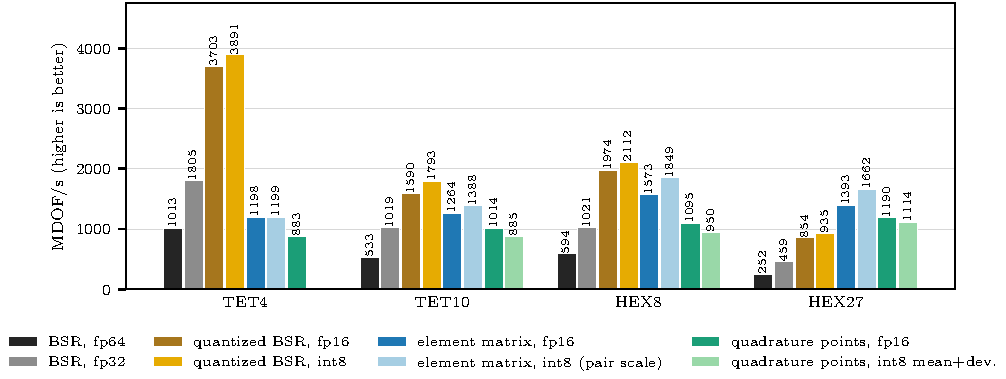
\includegraphics[width=0.85\textwidth]{throughput.pdf}
\caption{Application throughput, $\benchdofHexEight$~dof, $72$ threads.  TET4 has no
mean-and-deviation encodings: one point per element leaves no deviation.}
\Description{Grouped bar chart of million degrees of freedom per second for each format and
element.}
\label{fig:throughput}
\end{figure*}

\begin{figure*}[t]
\centering
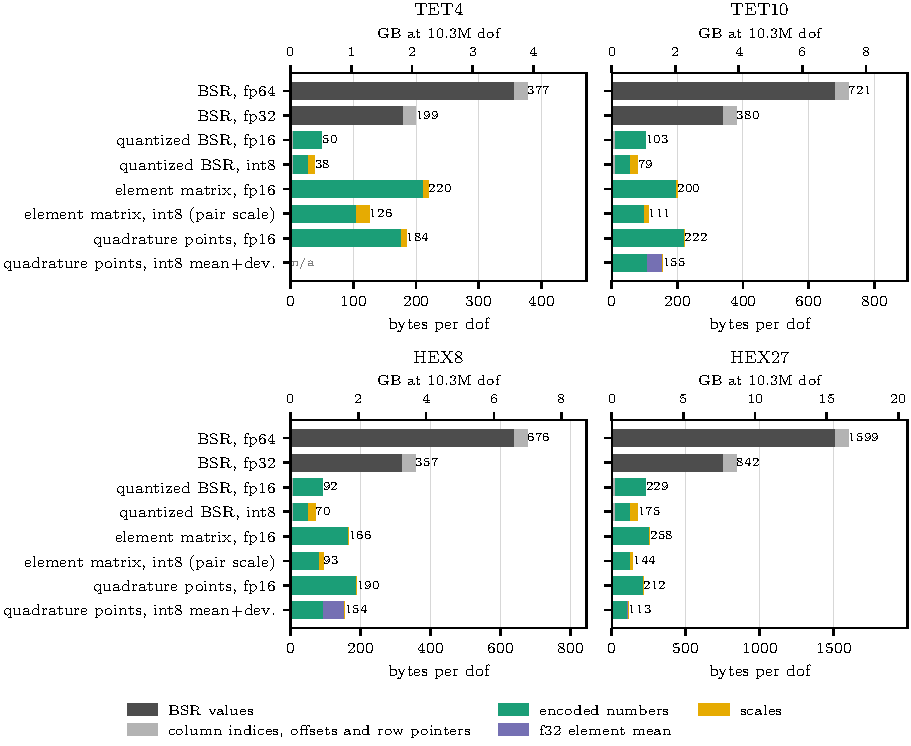
\includegraphics[width=0.8\textwidth]{memory_footprint.pdf}
\caption{Operator memory in bytes per degree of freedom (top axis: gigabytes at
$\benchdofHexEight$~dof), split into encoded numbers, indices and scales.}
\Description{Horizontal bar charts of operator memory per element type.}
\label{fig:memory}
\end{figure*}

BSR is at its bandwidth bound ($\bsrThirtyTwoRateHexEight$~MDOF/s on HEX8 in single precision,
Figure~\ref{fig:throughput}).  Of the element formats that keep the exact iteration counts, the
half-precision element matrix in difference form is the fastest, at $\EaDiffHalfVsThirtyTwoHexEight\times$,
$\EaDiffHalfVsThirtyTwoTetTen\times$ and $\EaDiffHalfVsThirtyTwoHexTwentySeven\times$ the speed of
single-precision BSR on HEX8, TET10 and HEX27; the half-precision point store reaches
$\QpHalfVsThirtyTwoHexEight$, $\QpHalfVsThirtyTwoTetTen$ and $\QpHalfVsThirtyTwoHexTwentySeven\times$.
On TET4, with two elements per degree of freedom and fifteen blocks per matrix row, every element
format is slower than BSR.  The quantized matrix is the fastest format on three of the four
elements: in \texttt{int8} it applies at $\QbsrEightVsThirtyTwoTetFour$, $\QbsrEightVsThirtyTwoTetTen$,
$\QbsrEightVsThirtyTwoHexEight$ and $\QbsrEightVsThirtyTwoHexTwentySeven\times$ the speed of
single-precision BSR from $\QbsrEightMemVsThirtyTwoTetTen$--$\QbsrEightMemVsThirtyTwoTetFour\times$ less
memory (Figure~\ref{fig:memory}).  Storing each pair once makes it
$\upperGainHexTwentySeven$--$\upperGainHexEight\times$ faster than the full difference form from
$\upperMemTetTen$--$\upperMemTetFour\times$ less memory, and the offsets save a further
$\offsetSavingHexEight\%$.  It is not bandwidth-bound --- $\gbsQbsrEightHexEight$~GB/s on HEX8 against
$\gbsBsrThirtyTwoHexEight$ for BSR --- because every stored block gathers its own $x_j$, which an
element format reads once per element node; on HEX27, with $\blocksHexTwentySeven$ blocks per row,
the element matrix with a scale per node pair stays ahead ($\EaPairEightRateHexTwentySeven$ against
$\QbsrEightRateHexTwentySeven$~MDOF/s).

\subsection{Newton iterations}

\begin{figure*}[t]
\centering
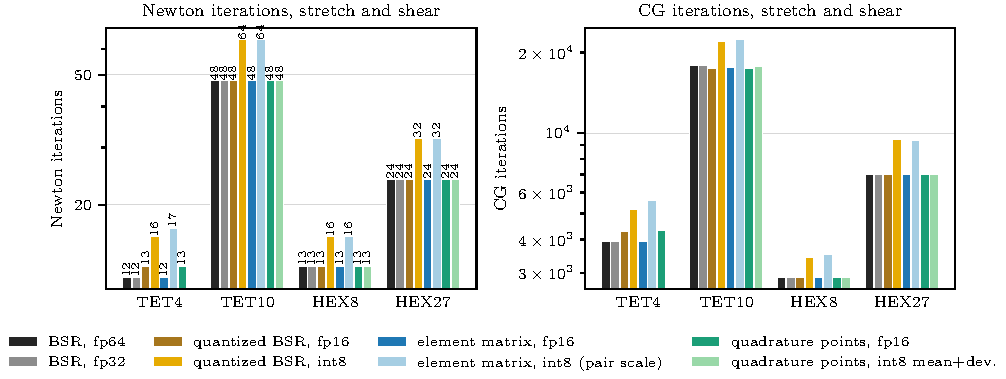
\includegraphics[width=0.85\textwidth]{newton_iterations.pdf}
\caption{Newton and CG iterations, about $10^6$~dof, log scale.  BSR in both precisions, the
matrix-free operator and the double-precision store have identical counts, shown once.  Encodings
with one \texttt{int8} scale per element are left out; their counts are in the text.}
\Description{Grouped bar charts of Newton and conjugate-gradient iteration counts.}
\label{fig:newton}
\end{figure*}

The iteration counts follow \eqref{eq:forcing} (Figure~\ref{fig:newton}).  The projected store costs
$\newtonPzeroExtraHexEight\%$ more Newton iterations on HEX8 and $\newtonPzeroExtraTetTen\%$ on TET10.
\texttt{int8} with one scale per element is not usable: the point store needs
$\newtonQpEightElTetTen$ Newton iterations on TET10 and $\newtonQpEightElHexEight$ on HEX8, against
$\newtonExactTetTen$ and $\newtonExactHexEight$.  The \texttt{int8} mean-and-deviation store keeps the
exact counts ($\newtonQpEightMdTetTen$ and $\newtonQpEightMdHexEight$), as do \texttt{fp16} and the
half-precision element matrix in difference form.  The quantized matrix needs the difference form:
encoded in full, in \texttt{int8} $\fullEightFailed$ of $\fullEightTried$ runs failed in the first load
step; in difference form in \texttt{fp16} it keeps the exact counts on HEX8, TET10 and HEX27
($\newtonQbsrHalfHexEight$, $\newtonQbsrHalfTetTen$, $\newtonQbsrHalfHexTwentySeven$), and in
\texttt{int8} with a scale per block it needs about a third more ($\newtonQbsrEightTetTen$ on TET10),
as the element matrix with a scale per node pair.

\subsection{Time to solution and peak memory}

\begin{figure*}[t]
\centering
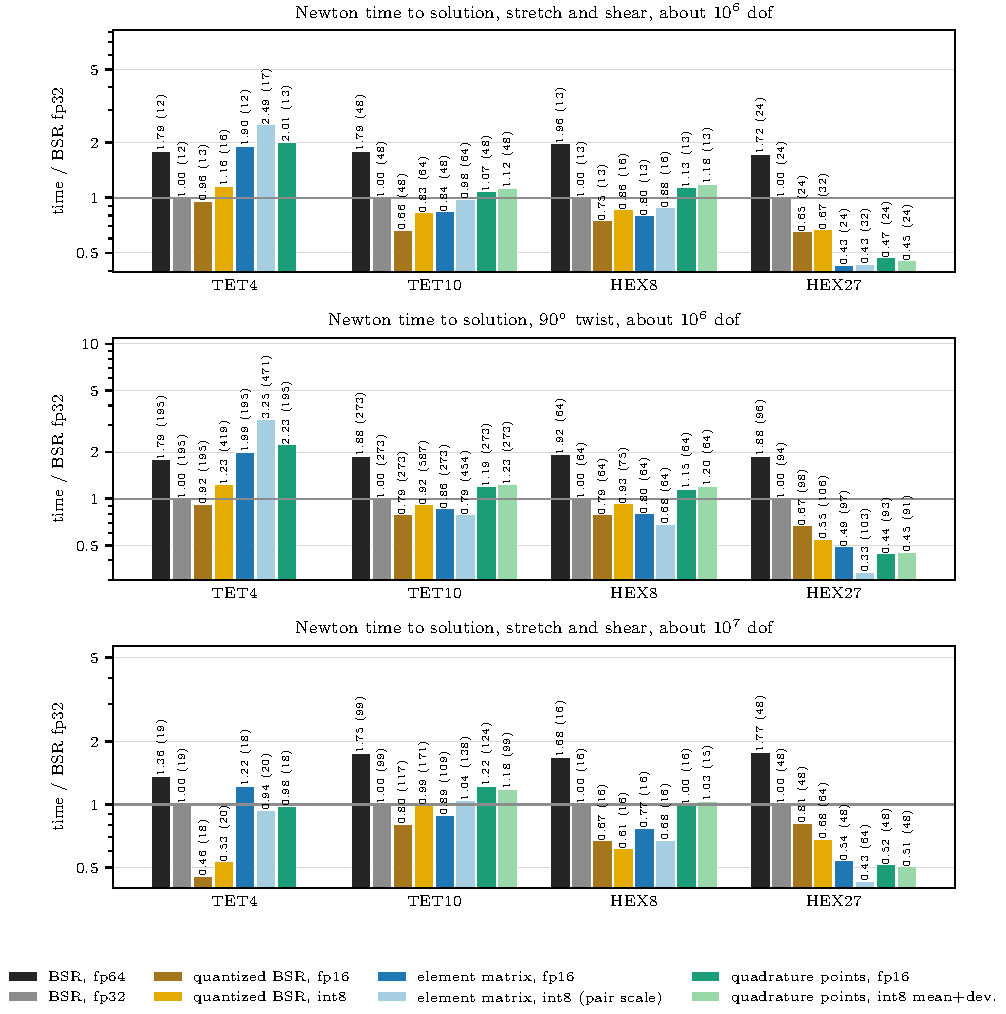
\includegraphics[width=0.85\textwidth]{time_to_solution.pdf}
\caption{Newton time to solution relative to single-precision BSR (log scale, below one is faster),
stretch at $10^6$ and $10^7$~dof and twist at $10^6$~dof; labels give the ratio and the Newton
iterations.  Failed load-step attempts are included in the time.}
\Description{Bar charts of time to solution relative to single-precision BSR for three cases.}
\label{fig:tts}
\end{figure*}

\begin{table*}[t]
\centering
\small
\begin{tabular}{lcccccc}
\toprule
 & \multicolumn{2}{c}{quantized BSR} & \multicolumn{2}{c}{element matrix} & \multicolumn{2}{c}{quadrature-point store} \\
\cmidrule(lr){2-3}\cmidrule(lr){4-5}\cmidrule(lr){6-7}
element & \texttt{fp16} & \texttt{int8} & \texttt{fp16} diff. & \texttt{int8} pair & \texttt{fp16} & \texttt{int8} mean+dev \\
\midrule
\rows{../tables/summary.tex}
\bottomrule
\end{tabular}
\caption{The evaluation in one table: Newton time to solution at about $10^7$ degrees of freedom
relative to single-precision BSR (stretch case), and in parentheses the factor by which the operator
is smaller than single-precision BSR.  The fastest format of each element in bold.}
\label{tab:summary}
\end{table*}

Table~\ref{tab:summary} and Figure~\ref{fig:tts} summarise the evaluation at about $10^7$ degrees of
freedom.  On the tetrahedra the \texttt{fp16} quantized matrix is the fastest format, at
$\timeQbsrHalfTetFour$ and $\timeQbsrHalfTetTen$ of the time of single-precision BSR; on TET10 it needs
$\tenmNewtonQbsrHalfTetTen$ Newton iterations against $\tenmNewtonExactTetTen$ and still wins on
application speed.  On HEX8 the \texttt{int8} quantized matrix and the element matrix with a scale per
node pair are close ($\timeQbsrEightHexEight$ and $\timeEaPairEightHexEight$).  On HEX27 every element
format beats the quantized matrix, and the pair-scaled element matrix is fastest at
$\timeEaPairEightHexTwentySeven$, with the quadrature-point stores close behind.

Operator memory is not peak memory.  The quantized matrix's application reads
$\storeQbsrEightHexEight$~GiB on HEX8 at $\peakDofHexEight$ degrees of freedom, but the whole Newton
run peaks at $\peakQbsrEightHexEight$~GiB against $\peakBsrThirtyTwoHexEight$ for single-precision BSR
and $\peakEaPairEightHexEight$ for the \texttt{int8} element matrix: the single-precision assembly and
the node graph it is built on set the peak.  The element formats need neither.

%% ===================================================================================================
\section{Discussion and conclusions}

The choice of format follows the element.  Where a matrix row has few blocks and the element formats
repeat each coupling in every element sharing it --- linear and quadratic tetrahedra --- the quantized
assembled matrix is the fastest format.  Where rows are long and elements large --- triquadratic
hexahedra --- the element formats win, because they gather each node once per element where the
matrix gathers it once per block.  Trilinear hexahedra sit between.  Across all elements the element
formats keep the lowest peak memory; assembling and encoding the matrix in chunks of rows would
close part of that gap.

Two properties decide which encodings are usable in a Newton iteration, for every format: the
rounding must follow the values or their variation over the element, not the largest entry of the
element, and the encoded operator must keep the rigid translations in its kernel.  Half precision and
\texttt{int8} mean-plus-deviation satisfy the first; the difference form provides the second and is
what makes \texttt{int8} usable for element and assembled matrices.  Storing what the quadrature sees
of the tangent, rather than its element average, removes the iterations the projection costs.

The gains need the operator to stream from memory: while the matrix fits in the last-level cache,
BSR is faster.  The study uses one material, structured meshes and an unpreconditioned Krylov
method; with a preconditioner built from the operator, the encodings change the preconditioner too.

\bibliographystyle{ACM-Reference-Format}
\bibliography{refs}

\end{document}
